% Source for the figure of SuffixTree (sec. 15.5): the suffix tree of
% banana$, the internal nodes with their string depth, the leaves with the
% start of their suffix, the edges with their labels, and the suffix links
% of the internal nodes (dashed). Build: make figures (in ../build).
\documentclass[border=4pt]{standalone}
\usepackage[T1]{fontenc}
\usepackage{newpxtext,newpxmath}
\usepackage[varqu,varl,scaled=0.95]{zi4}
\usepackage{tikz}
% tikz-ads.tex: the TikZ styles shared by the figures of the memory of the
% manual, \input by each standalone figure: a cell of a vector (cell), the
% cell that an operation touches (touched), a free cell (free), a node of a
% linked structure (node), the labels of indices (index) and of variables
% (var), a pointer (ptr), and \cells and \indices to draw a row of cells.
\usetikzlibrary{arrows.meta,positioning,calc,fit,shapes.multipart}
\definecolor{adsTouched}{RGB}{214,196,236}
\definecolor{adsFree}{RGB}{236,236,236}
\tikzset{
  ads/.style={>={Stealth[length=2mm]},font=\small,
              every node/.append style={inner sep=0pt}},
  cell/.style={draw,minimum width=7mm,minimum height=7mm,
               font=\small\ttfamily,outer sep=0pt},
  touched/.style={cell,fill=adsTouched},
  free/.style={cell,fill=adsFree,text=black!45},
  node/.style={draw,rounded corners=1pt,minimum width=8mm,
               minimum height=6mm,font=\small\ttfamily},
  index/.style={font=\scriptsize\ttfamily,text=black!60},
  var/.style={font=\small\itshape},
  ptr/.style={->,thick}
}
% \cells{name}{x,y}{list}: a row of cells, the first at (x,y), named
% name-0, name-1, ...; each item is text/style, the style one of cell,
% touched and free (e.g., {a/cell,e/touched,/free})
\newcommand{\cells}[3]{%
  \foreach \v/\s [count=\i from 0] in {#3}
    \node[\s] (#1-\i) at ($(#2)+(\i*7mm,0)$) {\v};}
% \indices{name}{n}: the indices 0 .. n-1 under the cells of name
\newcommand{\indices}[2]{%
  \foreach \i in {0,...,\numexpr#2-1\relax}
    \node[index,below=1.2mm of #1-\i] {\i};}

\tikzset{
  inn/.style={circle,draw,minimum size=6mm,font=\scriptsize},
  lf/.style={rectangle,draw,fill=adsTouched,minimum size=5mm,
             font=\small\ttfamily},
  lab/.style={font=\small\ttfamily,fill=white,inner sep=1pt},
  sl/.style={->,dashed,black!60}
}
\begin{document}
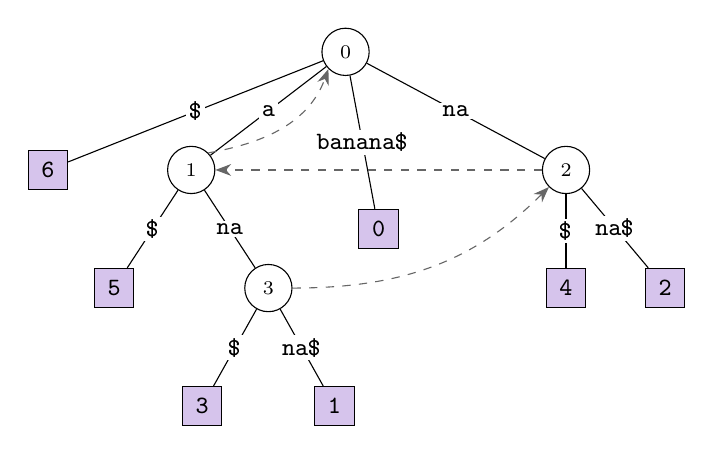
\begin{tikzpicture}[ads,x=14mm,y=15mm]
  \node[inn] (r)  at (3,0)    {0};
  \node[lf] (l6) at (0.3,-1) {6};
  \node[inn] (a)  at (1.6,-1) {1};
  \node[lf] (l0) at (3.3,-1.5) {0};
  \node[inn] (na) at (5,-1)   {2};
  \node[lf] (l5) at (0.9,-2) {5};
  \node[inn] (ana) at (2.3,-2) {3};
  \node[lf] (l3) at (1.7,-3) {3};
  \node[lf] (l1) at (2.9,-3) {1};
  \node[lf] (l4) at (5,-2) {4};
  \node[lf] (l2) at (5.9,-2) {2};
  \draw (r) -- node[lab] {\$} (l6);
  \draw (r) -- node[lab] {a} (a);
  \draw (r) -- node[lab] {banana\$} (l0);
  \draw (r) -- node[lab] {na} (na);
  \draw (a) -- node[lab] {\$} (l5);
  \draw (a) -- node[lab] {na} (ana);
  \draw (ana) -- node[lab] {\$} (l3);
  \draw (ana) -- node[lab] {na\$} (l1);
  \draw (na) -- node[lab] {\$} (l4);
  \draw (na) -- node[lab] {na\$} (l2);
  \draw[sl] (ana.east) to[out=0,in=-135] (na.south west);
  \draw[sl] (na.west) -- (a.east);
  \draw[sl] (a.north east) to[out=10,in=-110] (r.south west);
\end{tikzpicture}
\end{document}
